\section{Условие}
\textbf{Цель работы:} получить практические навыки управления потоками
операционной системы и синхронизации между ними.

\textbf{Задание:} разработать программу на языке C, обрабатывающую данные
в многопоточном режиме с помощью стандартных средств ОС. Максимальное число
одновременно работающих потоков задаётся ключом запуска. Необходимо показать
число потоков средствами ОС, исследовать зависимость ускорения и эффективности
от размера данных и числа потоков и объяснить результаты.

\textbf{Вариант 10:} решить систему линейных уравнений методом Гаусса.
Исходным заданием служит предоставленный PDF <<Лабораторная работа 3>>.
Дополнительно реализованы чтение системы из файла, воспроизводимая генерация,
проверка решения и демонстрационная пауза. Оформление адаптировано из шаблона
\href{https://github.com/Yadroff/OS_report_template}{Yadroff/OS\_report\_template}.
Отдельный Word-файл с требованиями к этой работе не был приложен.

\section{Метод решения}
Требуется найти вектор $x$ из равенства $Ax=b$, где $A$ --- квадратная матрица
размера $n$, а $b$ --- вектор правых частей. В памяти хранится расширенная
матрица $[A|b]$ размером $n\times(n+1)$, тип элементов --- \texttt{double}.
Индексы в формулах ниже, как и в C, начинаются с нуля.

На шаге $k$ прямого хода выбирается строка с наибольшим $|a_{ik}|$ среди
$i=k,\ldots,n-1$. Она переставляется с ведущей строкой $k$. Такой частичный
выбор главного элемента уменьшает опасность деления на очень малое число.
Для каждой строки $i>k$ вычисляется
\[
 m_i=\frac{a_{ik}}{a_{kk}},\qquad
 a_{ij}\leftarrow a_{ij}-m_i a_{kj},\quad j=k+1,\ldots,n.
\]
Элемент $a_{ik}$ становится нулём. Столбец $j=n$ --- свободные члены;
он изменяется вместе с коэффициентами. Эквивалентные преобразования строк
сохраняют решения системы. После прямого хода матрица коэффициентов
становится верхнетреугольной.

Обратный ход выполняется от последней строки к первой:
\[
 x_i=\frac{a_{i,n}-\sum_{j=i+1}^{n-1}a_{ij}x_j}{a_{ii}}.
\]
Последовательная версия использует тот же код исключения строк при одном
участнике. Основная трудоёмкость прямого хода --- $O(n^3)$, обратного ---
$O(n^2)$, память --- $O(n^2)$. Сохраняется копия исходной матрицы для проверки.

Порог ведущего элемента равен
$\varepsilon n\max_{i,j<n}|a_{ij}|$, где
$\varepsilon=\texttt{DBL\_EPSILON}$.
Если модуль опоры не превосходит порог или не является конечным числом,
решение прекращается. Так обнаруживаются вырожденность и часть численно
опасных случаев. Программа не различает несовместную систему и систему
с бесконечным числом решений: в обоих случаях безопасное единственное
решение недоступно. Это консервативный критерий, а не оценка числа
обусловленности; плохо масштабированная обратимая матрица тоже может быть отклонена.

\section{Многопоточный алгоритм и синхронизация}
Ключ \texttt{--threads P} задаёт верхнюю границу \emph{общего} числа потоков
процесса вместе с основным. Фактическое число участников $p=\min(P,n)$.
Создаются $p-1$ рабочих, основной поток имеет номер 0 и тоже обрабатывает строки.
При $P=1$ дополнительные потоки не создаются. Набор рабочих постоянный на
протяжении решения. Это исключает создание и завершение потоков на каждом шаге.

После выбора опоры остаётся $r=n-k-1$ строк. Участник с номером $t$ получает
полуоткрытый интервал
\[
\left[k+1+\left\lfloor\frac{rt}{p}\right\rfloor,
      k+1+\left\lfloor\frac{r(t+1)}{p}\right\rfloor\right).
\]
Интервалы не пересекаются и вместе покрывают все нижние строки. Число строк
у участников отличается максимум на одну. В конце алгоритма некоторые
интервалы пусты, но все рабочие подтверждают завершение шага.

Состояние набора потоков хранится в структуре \texttt{Pool}:
текущий шаг \texttt{k}, номер задания \texttt{generation}, счётчик
\texttt{done} и флаг \texttt{stop}. Эти поля защищены одним mutex.
Две условные переменные отвечают за новое задание (\texttt{work})
и завершение шага (\texttt{finished}).

Последовательность действий на шаге:
\begin{enumerate}[nosep]
\item Main выбирает и переставляет ведущую строку после завершения прошлого шага.
\item Под mutex записывает k, обнуляет done, увеличивает generation и будит рабочих.
\item Рабочие запоминают k под mutex, отпускают замок и обрабатывают свои строки.
Main одновременно вычисляет свой диапазон.
\item Рабочие под mutex увеличивают done. Последний будит main.
\item Main ждёт done=$p-1$, после чего может менять следующую ведущую строку.
\end{enumerate}
Все ожидания используют \texttt{while}: условие проверяется повторно после
пробуждения. Номер задания не даёт повторно выполнить старую работу.
Активного ожидания нет. Матрица во время исключения не блокируется:
каждый поток пишет только свои строки, ведущая строка доступна всем для чтения.
Mutex также обеспечивает видимость записей при передаче задания и завершения.
Поэтому нет одновременной записи в один элемент или смены опоры до окончания шага.

Нельзя одновременно выполнять все шаги k: строка следующей опоры зависит от
предыдущего исключения. Обратный ход также оставлен последовательным.
При завершении main устанавливает stop, будит рабочих и вызывает join для каждого.
Только затем уничтожаются средства синхронизации и освобождается память.

\section{Описание программы}
Вся реализация C находится в \texttt{main.c}; сборка задаётся \texttt{CMakeLists.txt}.
\texttt{Worker} содержит указатель на общий Pool и номер участника.
Матрица хранится непрерывно: элемент $(i,j)$ имеет индекс $i(n+1)+j$.
Проверяются выделение памяти, чтение, аргументы, результаты создания потоков,
опоры и конечность решения. При ошибке pthread\_create уже созданные рабочие
корректно завершаются. Для остальных ошибок pthread выводится код и процесс
завершается. Отказ ресурсов искусственно не провоцировался.

Основные функции: \texttt{generate} создаёт систему; \texttt{eliminate}
обрабатывает диапазон; \texttt{worker\_main} выполняет цикл рабочего;
\texttt{start\_pool}/\texttt{stop\_pool} управляют набором;
\texttt{gauss} выбирает опоры, согласует шаги и делает обратный ход;
\texttt{verify} проверяет ответ. Вспомогательные \texttt{number}, \texttt{help},
\texttt{seconds}, \texttt{known\_x}, \texttt{check\_pthread}
обслуживают ввод, время и ошибки. \texttt{main} связывает этапы.

Использованы функции POSIX Threads:
\begin{itemize}[nosep]
\item \texttt{pthread\_create}, \texttt{pthread\_join} --- запуск и ожидание завершения;
\item \texttt{pthread\_mutex\_init/lock/unlock/destroy} --- защита состояния;
\item \texttt{pthread\_cond\_init/wait/signal/broadcast/destroy} --- сон и пробуждение.
\end{itemize}
Это функции библиотечного интерфейса pthread, а не прямые системные вызовы
в исходном коде. \texttt{pthread\_barrier\_t} не используется, поскольку
он не подходит для выбранной переносимой реализации macOS.
Таймер --- \texttt{clock\_gettime(CLOCK\_MONOTONIC)}, пауза ---
\texttt{nanosleep}, PID --- \texttt{getpid}. Сторонних математических библиотек нет.

\section{Сборка и запуск}
Из корня проекта:
\begin{lstlisting}[language=bash,numbers=none,basicstyle=\small\ttfamily]
cmake -S . -B build -DCMAKE_BUILD_TYPE=Release \
  -DCMAKE_C_FLAGS_RELEASE='-O2 -DNDEBUG'
cmake --build build
./build/OS_Lab3_Variant10 --size 1000 --threads 4
./build/OS_Lab3_Variant10 --file tests/three.txt --threads 4
./build/OS_Lab3_Variant10 --help
\end{lstlisting}
В CLion нужно открыть корневую папку как CMake-проект и задать аргументы
в конфигурации запуска. Файл читается в формате: сначала N, затем N строк
по N коэффициентов и одному свободному члену. Ключи size/file взаимоисключающие.
Допустимы $1\le n\le10000$, $1\le P\le256$. Для $n=10000$ только две
матрицы занимают около 1,6 ГБ, а вычисление требует большого времени.
Для $n=1000$ две матрицы занимают примерно 15,3 МиБ.

Терминальная сборка CMake и тесты подтверждены. Проект открыт в CLion, исходный файл отображается, CMake загрузился.
Глобальный профиль IDE использует GCC 16. Для Apple Clang добавлен отдельный
preset apple-clang (CMake 3.21+), его сборка через CMake проверена.
После повторной сборки кнопкой Build в CLion получено сообщение
Build finished. Сборка IDE проверена в исходном профиле Debug с GCC 16.2.0;
основные тесты и замеры выполнены Apple Clang. Глобальные настройки IDE
не менялись, preset Apple Clang загружен отдельно.
Исходный код использует переносимые интерфейсы C11 и POSIX; в Linux CMake
дополнительно подключает стандартную libm. Запуск и сборка в Ubuntu в этой
сессии не выполнялись: готовой работающей Linux-среды не было. Виртуальная
машина не устанавливалась.

\section{Проверка корректности и примеры}
Тестовая система из \texttt{tests/three.txt}:
\[
\begin{cases}
2x_1+x_2-x_3=8,\\
-3x_1-x_2+2x_3=-11,\\
-2x_1+x_2+2x_3=-3.
\end{cases}
\]
Найдено $x=(2,3,-1)$. При разных лимитах потоков значения совпали с учётом
погрешности; для маленьких примеров совпали и напечатанные значения double.
Реальный вывод программы:
\par\medskip
\begin{minipage}{\textwidth}
\lstinputlisting[language={},numbers=none,basicstyle=\small\ttfamily]{../results/example.txt}
\end{minipage}
\par\medskip

Сгенерированные матрицы строго диагонально преобладающие.
Линейный конгруэнтный генератор имеет фиксированное начальное состояние 10
и арифметику uint32\_t. Эталон $x_j=(j\bmod7)-3$, а $b$ вычисляется как
$Ax_{ref}$. Для одного n во всех запусках получаются одинаковые исходные данные.

Проверяется абсолютная невязка $\|Ax-b\|_\infty$ и относительная величина
\[
\eta=\frac{\|Ax-b\|_\infty}
{\|A\|_\infty\|x\|_\infty+\|b\|_\infty}\le10^{-10}.
\]
Здесь $\|A\|_\infty$ --- максимальная сумма модулей элементов строки.
Для нулевого знаменателя проверяется сама невязка, переполнение даёт отказ.
Для генератора дополнительно требуется $\max_j|x_j-x_{ref,j}|\le10^{-8}$.
Малая невязка не гарантирует малую ошибку x у плохо обусловленной системы.
На Apple arm64 тип long double не даёт гарантированного преимущества
точности по сравнению с double; проверка на это преимущество не опирается.

\begin{center}
\begin{tabular}{p{10.7cm}r}
\hline
Группа проверок & Число\\\hline
Известные ответы: 2, 3 и 1 неизвестная, pivot, масштаб $10^{-100}$,
нулевая правая часть; лимиты 1/2/4/8 & 24\\
Ошибочные и вырожденные файлы; лимиты 1/4 & 18\\
Генерация: n=1,2,3,7,10,31,100,300,600,1000; 1/2/4/8 & 40\\
Некорректные аргументы и справка & 17\\
Повторные многопоточные решения n=31, p=8 & 25\\\hline
Всего на одну сборку & 124\\\hline
\end{tabular}
\end{center}
Все 124 проверки пройдены в Release, под AddressSanitizer вместе с
UndefinedBehaviorSanitizer и отдельно под ThreadSanitizer.
Диагностик санитайзеров не получено. Три теста CTest также прошли.
Журналы сохранены в \texttt{report/results/*-tests.json}.
Проверка отсутствия гонок дополнена анализом непересекающихся диапазонов
и синхронизации шагов; результат TSan не является доказательством для всех входов.
Ошибки malloc и pthread\_create проверены в коде, но не вызывались
искусственным исчерпанием памяти или лимита потоков.

\section{Демонстрация числа потоков}
Для наблюдения используется отдельная пауза после создания рабочих и до таймера:
\begin{lstlisting}[language=bash,numbers=none,basicstyle=\small\ttfamily]
./build/OS_Lab3_Variant10 --size 1000 --threads 4 --demo 20 &
pid=$!
ps -M -p "$pid"
wait "$pid"
\end{lstlisting}
В macOS команда проверена на реальных процессах. После заголовка ps показывает
по строке на поток. Во время демопаузы потоки спят, а затем тот же набор
потоков выполняет решение. Пауза не входит в измеряемое время.

\begin{center}
\begin{tabular}{rrrr}
\hline n & Лимит P & Наблюдалось потоков & Проверка\\\hline
100 & 1 & 1 & пройдена\\
100 & 2 & 2 & пройдена\\
100 & 4 & 4 & пройдена\\
100 & 8 & 8 & пройдена\\
3 & 8 & 3 & пройдена\\\hline
\end{tabular}
\end{center}
Ниже приведён настоящий вывод для P=4. Из длинной первой строки убран только
путь COMMAND для читаемости; числовые поля сохранены, полный журнал лежит
в \texttt{threads-p4-n100.txt}. Это текстовый снимок, а не изображение терминала.
\lstinputlisting[language={},numbers=none,basicstyle=\footnotesize\ttfamily]{../results/ps-fragment.txt}
Отдельный скриншот демонстрации терминала не сохранён. Вместо изображения
сохранены исходные
логи ps для всех пяти случаев и итоговая таблица JSON.
Для Ubuntu подготовлена команда \texttt{ps -T -p "\$pid"}; на Ubuntu она
в этой сессии не проверялась. Вывод strace не приводится: на macOS он не запускался.

\section{Исследование производительности}
Эксперимент выполнен 19.10.2026 непосредственно на MacBook с Apple M1,
8 ГиБ оперативной памяти; macOS 26.5.1 (25F80), arm64. По sysctl доступны
8 физических и 8 логических ядер. Компилятор --- Apple Clang 21.0.0
(clang-2100.0.123.102), сборка CMake Release с \texttt{-O2 -DNDEBUG}.
Санитайзеры в измерениях отключены. Реальная конфигурация и SHA-256 исходника
сохранены в \texttt{environment.json}.

Исследованы n=100,300,600,1000 и p=1,2,4,8. Здесь p включает main и совпадает
с фактическим числом участников, поскольку во всех опытах n больше p.
Основной поток выполняет вычисления. В конце прямого хода некоторые
участники получают пустой диапазон; p означает выделенное число участников,
а не гарантированную постоянную занятость каждого.

Для каждой пары выполнен один прогрев и семь учитываемых запусков.
Конфигурации перемешаны с фиксированным seed. Одновременно выполнялся один
измеряемый процесс; санитайзеры и сборки к этому моменту завершились.
Обычные приложения macOS оставались открыты, привязка к ядрам и частоты
не управлялись. Поэтому результаты отражают эту рабочую среду и имеют разброс.

Монотонный таймер охватывает всю функцию gauss: выбор опоры, перестановки,
исключение строк, синхронизацию и обратный ход. Ввод, генерация, копирование
матрицы, создание/завершение набора потоков, проверка, печать и демопауза исключены.
Методика одинакова при любом p. Это время решения с готовым набором потоков,
а не полное время процесса. Итоговое время --- медиана семи наблюдений.
Всего сохранено 112 учитываемых измерений и выполнено 16 прогревов.

Ускорение и эффективность рассчитаны для каждого размера отдельно:
\[
 S(p)=\frac{T(1)}{T(p)},\qquad E(p)=\frac{S(p)}{p}.
\]
\begin{center}
\begin{tabular}{rrrrrr}
\hline
$n$ & $p$ & $T$, мс & min--max, мс & $S(p)$ & $E(p)$, \%\\\hline
100 & 1 & 0.169 & 0.149--0.182 & 1.000 & 100.00 \\
100 & 2 & 0.987 & 0.830--1.035 & 0.171 & 8.56 \\
100 & 4 & 1.536 & 1.255--1.879 & 0.110 & 2.75 \\
100 & 8 & 3.423 & 2.662--3.927 & 0.049 & 0.62 \\
300 & 1 & 4.206 & 3.673--4.852 & 1.000 & 100.00 \\
300 & 2 & 5.421 & 4.800--7.034 & 0.776 & 38.79 \\
300 & 4 & 7.024 & 5.495--7.494 & 0.599 & 14.97 \\
300 & 8 & 10.037 & 9.444--10.905 & 0.419 & 5.24 \\
600 & 1 & 32.494 & 28.901--37.692 & 1.000 & 100.00 \\
600 & 2 & 24.746 & 21.333--25.072 & 1.313 & 65.66 \\
600 & 4 & 25.066 & 19.864--28.772 & 1.296 & 32.41 \\
600 & 8 & 29.097 & 25.483--34.498 & 1.117 & 13.96 \\
1000 & 1 & 144.897 & 133.525--160.774 & 1.000 & 100.00 \\
1000 & 2 & 93.231 & 83.296--96.703 & 1.554 & 77.71 \\
1000 & 4 & 74.512 & 65.198--78.775 & 1.945 & 48.62 \\
1000 & 8 & 75.963 & 71.031--90.424 & 1.907 & 23.84 \\
\hline
\end{tabular}
\end{center}
Все времена в таблице указаны в миллисекундах. Исходные данные: raw.csv; агрегированные значения: summary.csv.


\clearpage
\section{Графики результатов}
\begin{center}
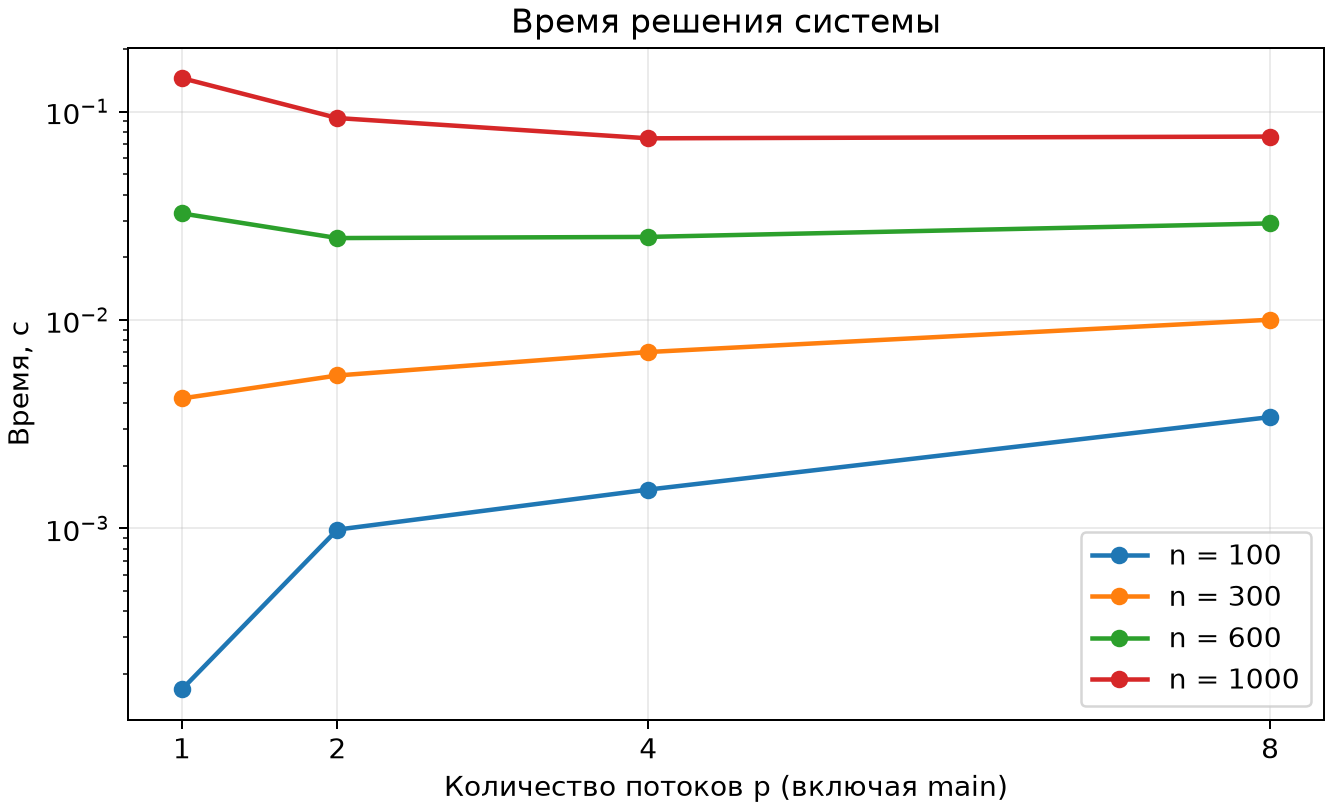
\includegraphics[width=\textwidth]{../results/time.png}

Время решения от числа потоков. Ось времени логарифмическая,
чтобы одновременно были видны все четыре размера.

\vspace{8pt}
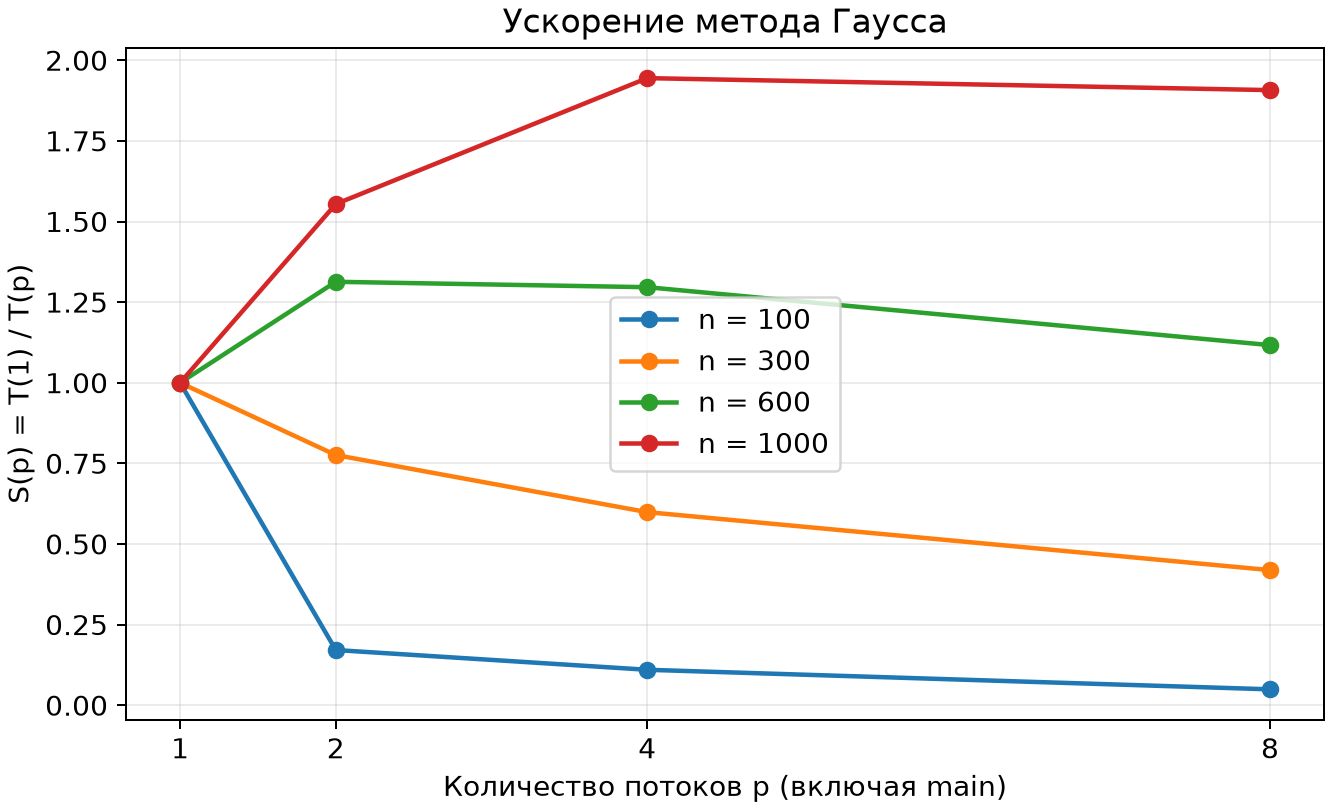
\includegraphics[width=\textwidth]{../results/speedup.png}

Ускорение относительно одного потока для каждого n.
\end{center}
\clearpage
\begin{center}
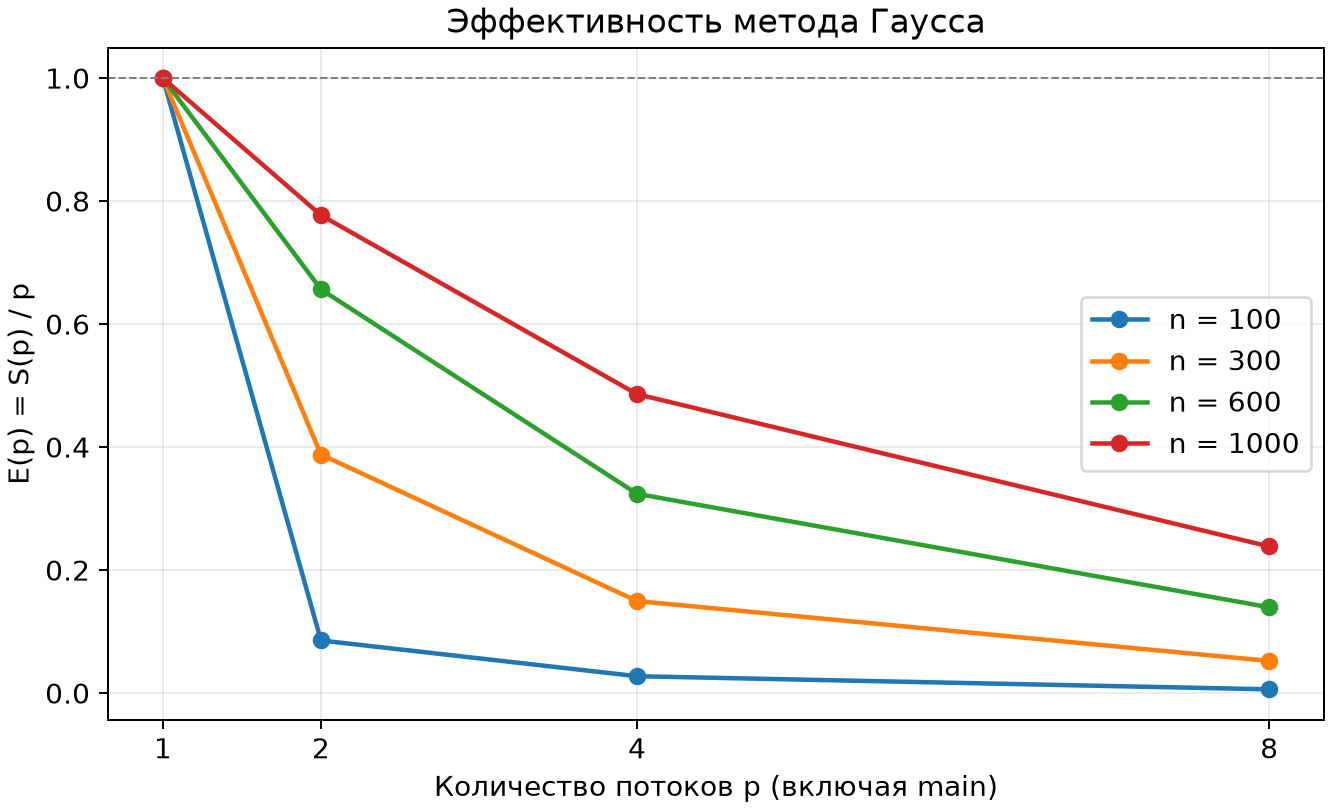
\includegraphics[width=\textwidth]{../results/efficiency.png}

Эффективность как доля от идеальной загрузки p участников.
\end{center}

\section{Анализ результатов}
При n=100 последовательное решение занимает около 0,169 мс. Для четырёх
потоков время 1,536 мс, ускорение 0,110: решение медленнее примерно в 9,09 раза.
Работы в отдельных строках мало, а ожидание, пробуждение и блокировки
требуются почти на каждом шаге. Постоянный набор устраняет повторные create/join,
но не устраняет эти расходы. При n=300 многопоточность тоже медленнее.

При n=600 два потока дают ускорение около 1,313, четыре --- 1,296.
При n=1000 время уменьшается с 0,144897 с до 0,074512 с на четырёх потоках:
$S(4)\approx1,945$, $E(4)\approx0,486$, то есть около 48,6\%.
Восемь потоков дают $S(8)\approx1,907$ и $E(8)\approx0,238$.
Разница медиан для четырёх и восьми потоков невелика, а интервалы
минимума--максимума пересекаются; строгий вывод о превосходстве четырёх
потоков при любой фоновой нагрузке делать нельзя.

У больших матриц объём вычислений растёт как $O(n^3)$, и расходы ожидания
лучше окупаются. Линейного ускорения нет: выбор опоры и обратный ход
последовательны, каждый шаг требует согласования, число нижних строк
уменьшается, а память и вычислительные ресурсы общие. Размещение потоков
планировщиком и фоновые задачи также могут влиять на время. Частоты, нагрузка
по конкретным ядрам и вклад каждого фактора отдельно не измерялись.
Наличие восьми физических ядер само по себе не обещает ускорения в восемь раз.

\section{Выводы}
Реализован метод Гаусса с частичным выбором ведущего элемента на C11
и переносимой синхронизацией pthread. Основной и рабочие потоки действительно
обрабатывают разные строки. Лимит потоков соблюдается и подтверждён ps.
Проверены известные решения, перестановки, вырожденные и ошибочные системы;
ASan/UBSan и TSan прошли выполненные тесты без диагностик.

Многопоточность полезна при достаточном объёме работы. В этой серии опытов
при n=1000 четыре потока дали ускорение около 1,94, а маленькие матрицы
выгоднее решать одним потоком. Измерения, графики и исходный код сохранены
для повторения. Неподтверждённые проверки: запуск и команда ps на Ubuntu,
искусственные отказы ресурсов. Скриншот терминала
заменён настоящими текстовыми журналами. Личные данные титульного листа
необходимо заполнить перед сдачей.

\section{Источники}
\begin{enumerate}[nosep]
\item Предоставленное задание <<Лабораторная работа 3.pdf>>, вариант 10.
\item Шаблон преподавателя:
\url{https://github.com/Yadroff/OS_report_template}. Просмотрен 19.10.2026.
\item Исходный код main.c и журналы экспериментов report/results данного проекта.
\end{enumerate}

\clearpage
\section{Исходная программа}
Полный код C11 из main.c. Номера строк соответствуют исходному файлу.
\lstinputlisting[language=C,basicstyle=\scriptsize\ttfamily,numbers=left,
numberstyle=\tiny,numbersep=7pt,xleftmargin=18pt,breaklines=true,columns=fullflexible]{../../main.c}
